\documentclass[12pt]{beamer}
\usepackage[table,xcdraw]{xcolor}
\usetheme{Madrid}
\usecolortheme{default}
\definecolor{meuazul}{RGB}{36, 150, 200}
\setbeamercolor{structure}{fg=meuazul}

\usepackage{ragged2e}
\usepackage[utf8]{inputenc}
\usepackage[brazil]{babel}
\usepackage[T1]{fontenc}
\usepackage{amsmath}
\usepackage{amsfonts}
\usepackage{amssymb}
\usepackage{graphicx}
\usepackage{setspace}
\setbeamertemplate{caption}[numbered]
\usepackage{hyperref}
\setbeamercovered{transparent} 
\setbeamertemplate{navigation symbols}{}
\usepackage[table,xcdraw]{xcolor}
\usepackage{ragged2e}

%referência e citação

\usepackage[backend=biber]{biblatex}
\addbibresource{ref.bib}



\addtobeamertemplate{block alerted}{}{\justifying}

\author[Prof. Fábio Rivas \& Joao Victor]{% 
Fábio Rivas\inst{1} \and Joao Victor\inst{2}}
\title[Triângulos, ruas e macarrão]{Triângulos, ruas e macarrão: o sabor da desigualdade (triangular)}
\institute[]{% 
  \textsuperscript{1} Professor \\
  \textsuperscript{2} Discente, Licenciatura em Matemática
}

\titlegraphic{
\includegraphics[width=0.2\textwidth]{imagens/logo_3.jpg}}
\date{\today} 


%\subject{}

% ---------------------------------------------------------

\begin{document}
\onehalfspacing 
\justifying 

\begin{frame}
    \titlepage
\end{frame}

\begin{frame}{Sumário}
    \tableofcontents
\end{frame}

\section{Desigualdade}

    \begin{frame}{Desigualdade}
        \begin{alertblock}{Definição - Dicionário Michaelis}
        \justifying
        
            \textbf{(1)} Atributo de pessoas ou coisas distintas; dessemelhança, diferença.\\
            \uncover<2->{\textbf{(2)} Falta de equilíbrio; disparidade, distância.}\\
            \uncover<3->{\textbf{(3)} Comparação de duas quantidades desiguais, em uma expressão matemática, através de sinais (maior, menor, diferente).} \\
        \end{alertblock}

        \uncover<4->{

        \begin{block}{Aplicação}
            Joao, um amante de pizza, decidiu fazer um rolé gastronômico por Manaus para encontrar a MELHOR pizza de frango com catupiry da cidade!
        \end{block}}

        
    \end{frame}

    \begin{frame}{A Grande Descoberta Matemática de Joao}
    
        \begin{columns}
        \begin{column}{0.6\textwidth}
       
            \textbf{Pizzaria A - Ingredientes}

            \begin{itemize}
                \item [1.] 300g de frango temperado
                \item [2.] 200g de catupiry cremoso
                \item [3.] 150g de molho de tomate caseiro
                \item [4.] 100g de mussarela derretida
                \item [5.] 50g de milho verde
                \item [6.] 30g de azeitonas pretas
                \item [7.] 20g de orégano fresco
            \end{itemize}
            
        \end{column}

        \begin{column}{0.4\textwidth}
            \centering
            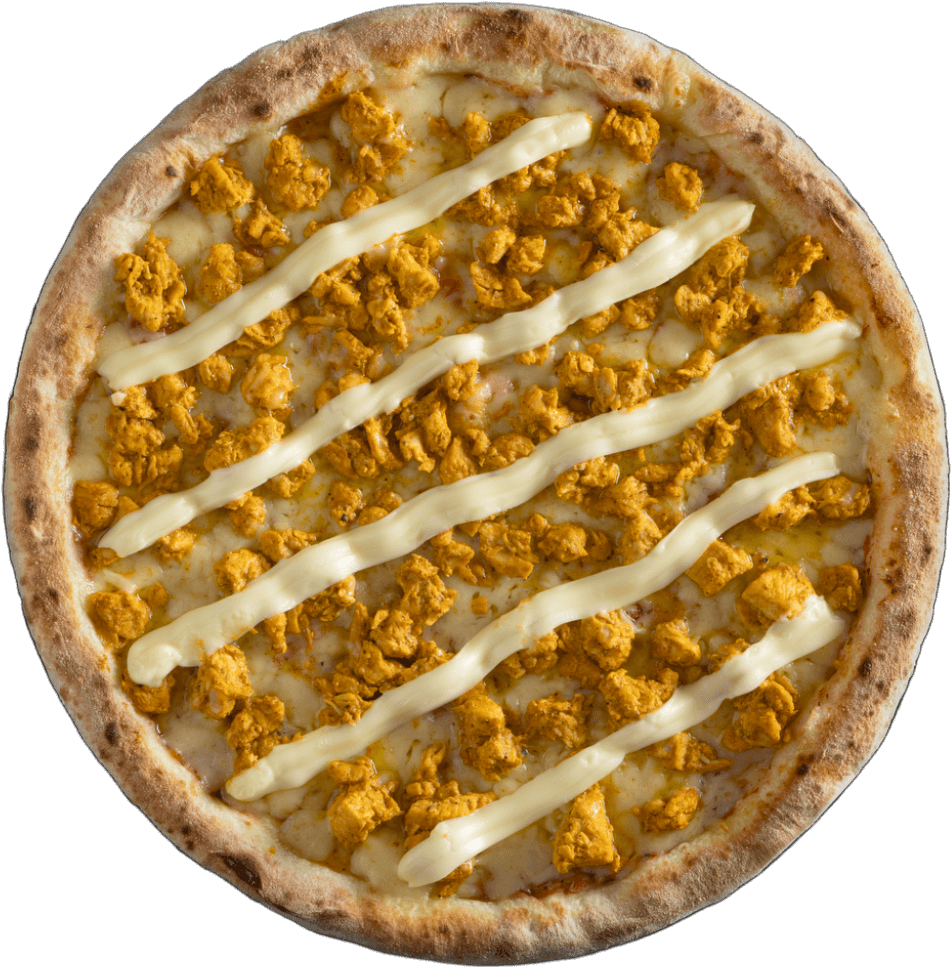
\includegraphics[width=0.8\linewidth]{imagens/pizza_1.png}
        \end{column}
    \end{columns}
        
    \end{frame}

    \begin{frame}{A Grande Descoberta Matemática de Joao}
    
        \begin{columns}
        \begin{column}{0.6\textwidth}
       
            \textbf{Pizzaria B - Ingredientes}

            \begin{itemize}
                \item [1.] 250g de frango temperado
                \item [2.] 250g de catupiry cremoso
                \item [3.] 120g de molho de tomate caseiro
                \item [4.] 120g de mussarela derretida
                \item [5.] 40g de milho verde
                \item [6.] 30g de azeitonas pretas
                \item [7.] 25g de orégano fresco
            \end{itemize}
        \end{column}

        \begin{column}{0.4\textwidth}
            \centering
            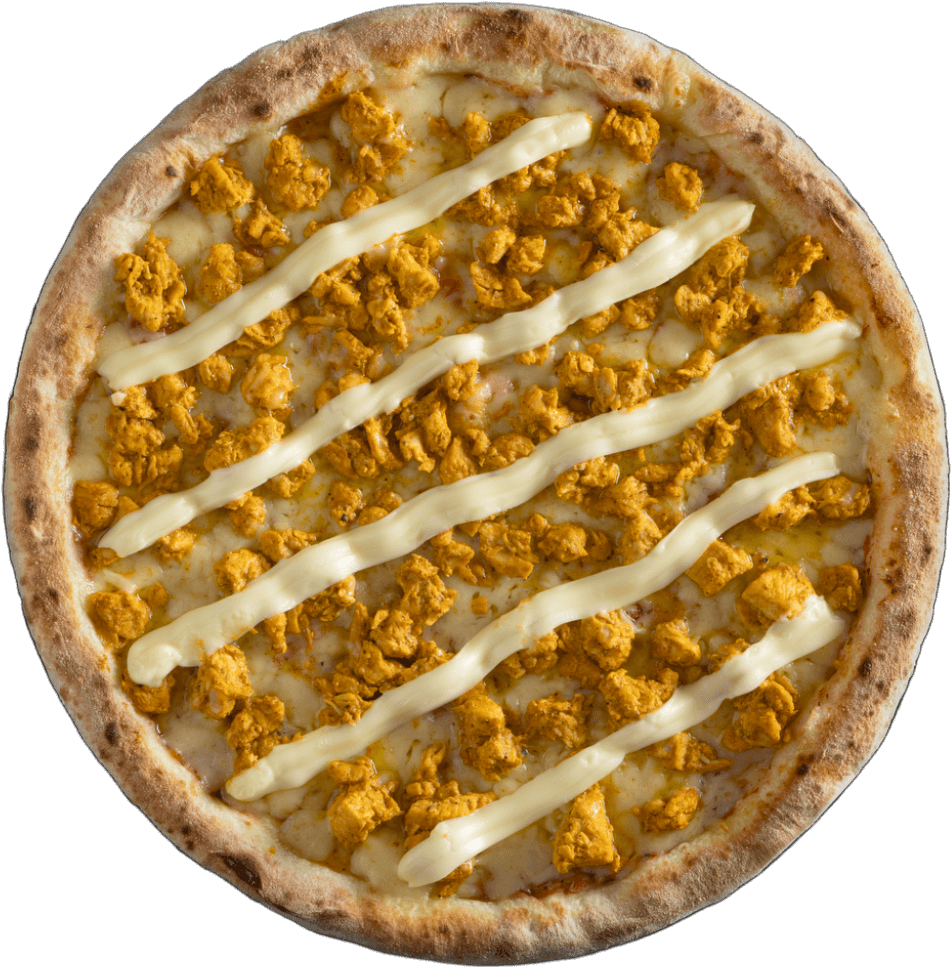
\includegraphics[width=0.8\linewidth]{imagens/pizza_1.png}
        \end{column}
    \end{columns}
        
    \end{frame}
    
    \begin{frame}{Comparando os ingredientes}
    
        \begin{table}[h]
        \centering
        \small
        \renewcommand{\arraystretch}{1.3}
            \begin{tabular}{lccc}
                \hline
                \textbf{Ingredientes (g)} & \textbf{Pizzaria A} & \textbf{Pizzaria B} & \textbf{A vs B} \\
                \hline
                Frango Temperado & 300 & 250 & 50g a mais \\
                Catupiry cremoso & 200 & 250 & 50g a menos \\
                Molho de tomate caseiro & 150 & 120 & 30g a mais \\
                Mussarela derretida & 100 & 120 & 20g a menos \\
                Milho verde & 50 & 40 & 10g a mais \\
                Azeitonas pretas & 30 & 30 & IGUAIS \\
                Orégano fresco & 20 & 25 & 5g a menos \\
                \hline
            \end{tabular}
        \end{table}

    \end{frame}
    
\section{Triângulo}

    \begin{frame}{Triângulo}
        \begin{alertblock}{Definição}
        \justifying
            \textbf{(1)} Polígono de três lados; trilátero.\\
            \uncover<2->{\textbf{(2)} Qualquer objeto que tenha formato triangular.}\\
            \uncover<3->{\textit{\textbf{(3)} Dados três pontos, A, B e C, não colineares, à reunião dos segmentos $\overline{AB}$, $\overline{BC}$ e $\overline{AC}$, chama-se \textbf{triângulo ABC} (Fundamentos de Matemática Elementar, volume 9)}}\\
        \end{alertblock}
    \end{frame}

    \begin{frame}{Tipos de triângulos}
        Quanto aos lados, os triângulos se classificam em:

        \begin{center}
            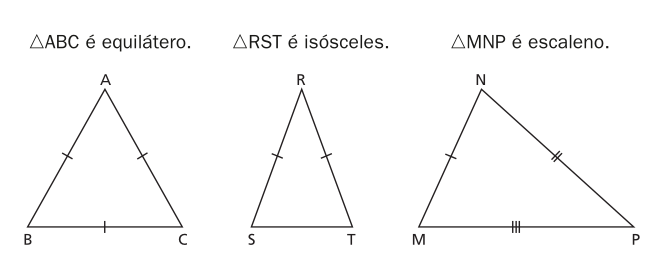
\includegraphics[scale=0.5]{imagens/triangulos.png}
        \end{center}
    \end{frame}
\section{Desigualdade Triangular}

    \begin{frame}{Desigualdade triangular}
        \begin{alertblock}{Definição}
        \justifying
            Em todo triângulo, a soma dos comprimentos de dois lados é maior que o comprimento do terceiro lado. 
        \end{alertblock}
        
        \pause
        
        \begin{block}{Aplicação}
            Existe triângulo cujos lados medem 5, 8 e 16? Por quê?
        \end{block}

    \end{frame}
    
\section{Verificação: é triângulo?}

    \begin{frame}{Probabilidade Geométrica - Problema do macarrão}
    \begin{minipage}{\textwidth}
        \centering
        \fbox{\begin{minipage}{0.9\textwidth}
            \vspace{0.3cm}
            \footnotesize
            
            \textbf{O grande desafio:} \\
            1. Pegue UM fio de espaguete \\
            2. QUEBRE-EM em 3 partes \textbf{arbitrariamente} \\
            3. Meça os comprimentos \textbf{a, b, c} \\
            4. Teste as desigualdades (marque \checkmark\ ou $\times$) \\
            5. Agora tente FORMAR o triângulo \\
            6. Se \textbf{TODAS} as desigualdades forem verdadeiras $\rightarrow$ triângulo possível! \\
            7. Se \textbf{UMA} for falsa $\rightarrow$ triângulo impossível! \\
            
            \textbf{Consegue prever antes de tentar montar?} \\
            \textbf{Regra da Desigualdade Triangular:} \\
            $a + b > c$ \textbf{e} $a + c > b$ \textbf{e} $b + c > a$
            \vspace{0.3cm}
        \end{minipage}}
    \end{minipage}
\end{frame}

    \begin{frame}{Aplicação em sala}
        \begin{table}[h]
        \centering
        \small
        \setlength{\tabcolsep}{8pt}
        \renewcommand{\arraystretch}{1.5}

            \begin{tabular}{|c|c|c||c|c|c||c|}
                \hline
                \textbf{a} & \textbf{b} & \textbf{c} & \textbf{a + b > c} & \textbf{a + c > b} & \textbf{b + c > a} & \textbf{Triângulo?} \\
                \hline
                & & & $\square$ & $\square$ & $\square$ & \\
                \hline
                & & & $\square$ & $\square$ & $\square$ & \\
                \hline
                & & & $\square$ & $\square$ & $\square$ & \\
                \hline
                & & & $\square$ & $\square$ & $\square$ & \\
                \hline
                & & & $\square$ & $\square$ & $\square$ & \\
                \hline
                & & & $\square$ & $\square$ & $\square$ & \\
                \hline
            \end{tabular}
        \end{table}
    \end{frame}

\section{Problema, probleminhas e \textit{problemão} (OBMEP)}




\begin{frame}{Probleminha: Quem andou mais?}

    \begin{exampleblock}{\textbf{Desafio 01.}}
        Ruas retas e compridas ligam as casas dos amigos Bruno, Francimar e Robério.

    \begin{itemize}\justifying
        \item Francimar, em sua caminhada matinal, saiu de sua casa e andou até a casa de Bruno. Em seguida, prosseguiu para a casa de Robério e depois voltou para sua casa.
        \item Mais tarde, Robério, muito concentrado com um problema de matemática, foi até a casa de Bruno e voltou para sua casa.
    \end{itemize} Sem conhecer as distâncias entre as casas, é possível saber quem andou mais?
    
    \end{exampleblock}

\end{frame}

\begin{frame}{Probleminha: Brincando com lápis}
	
	\begin{exampleblock}{\textbf{Desafio 02.}}
		\justifying
		Ana Paula tinha 2 lápis em mãos, cujos comprimentos eram de 5,8 cm e 11,4 cm, respectivamente. Com esses 2 lápis e um terceiro, entre os que tinha em seu estojo, ela começou a formar triângulos que tivessem os seus lápis como lados. Logo ela percebeu que com alguns dos lápis do estojo não era possível formar um triângulo. 
		
		\vspace{2mm} 
		
		Determine para que comprimentos do terceiro lápis Ana Paula conseguirá formar um triângulo.
	\end{exampleblock}
	
\end{frame}

\begin{frame}{Problema de Gincana: Isso não é perímetro}
	\begin{exampleblock}{\textbf{Desafio 03.}}
		Se $\overline{AB}+\overline{BC}=18$, então o perímetro do triângulo $ABC$ \textbf{NÃO} pode ser:
		
		\begin{itemize}
			\item [a)] 33
			\item [b)] 34
			\item [c)] 35
			\item [d)] 36
			\item [e)] Nenhuma das respostas anteriores
		\end{itemize}
	\end{exampleblock}
	
\end{frame}


\begin{frame}{Unicamp - 2024}

    \begin{exampleblock}{\textbf{Desafio 04.}}
        \justifying
        Joaquim estava brincando com um graveto, quando acertou uma parede e o graveto se partiu em três pedaços, de comprimentos a, b, c, com $a \leq b \leq c$. Ele recolheu os pedaços e tentou construir um triângulo cujos lados seriam exatamente os pedaços do graveto: \textbf{não foi possível}. Sabendo que o graveto tinha $50\ cm$ de comprimento e que $b = a + 2$, qual é o maior valor possível de a?

        \begin{itemize}
        \item [a)] 9,5 cm
        \item [b)] 10,5 cm
        \item [c)] 11,5 cm %
        \item [d)] 12,5 cm
    \end{itemize}

    \end{exampleblock}
   
\end{frame}

\begin{frame}{Problemão: Probabilidade com macarrão}

    \begin{exampleblock}{\textbf{Desafio 05.}}
        \justifying
        Quebrando aleatoriamente um macarrão, de tamanho qualquer, em três partes, qual a probabilidade de que elas possam formar um triângulo?

        \begin{center}
            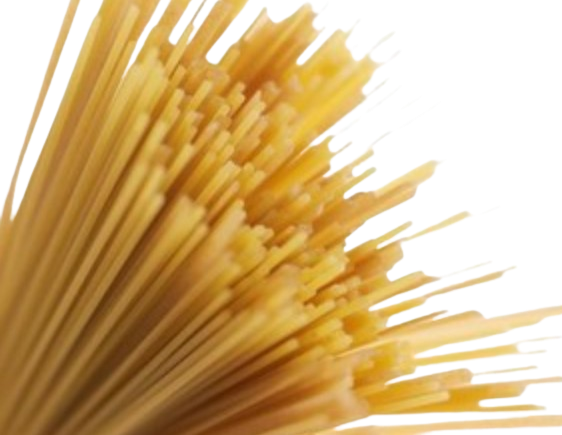
\includegraphics[scale=0.3]{imagens/macarrao_rmvbg.png}
        \end{center}
    
    \end{exampleblock}
   
\end{frame}


\begin{frame}{Referências}
	\justifying
	\begin{itemize}
		\item Clube de Matemática da OBMEP. \textbf{Probleminha: Quem andou mais?}. Disponível em: $<\href{https://clubes.obmep.org.br/blog/problema-quem-andou-mais/}{Desafio\  01.}>$
		
		\item Clube de Matemática da OBMEP. \textbf{Probleminha: Brincando com lápis}. Disponível em: $<\href{https://clubes.obmep.org.br/blog/probleminha-brincando-com-lapis/}{Desafio\  02}>$
		
		\item Clube de Matemática da OBMEP. \textbf{Problema de Gincana: Isso não é perímetro}. Disponível em: $<\href{https://clubes.obmep.org.br/blog/problema-de-gincana-isso-nao-e-perimetro/}{Desafio\  03}>$
		
		\item Elite Resolve. \textbf{Unicamp}. Disponível em: $<\href{https://sisq.elitecampinas.com.br/GabaritoVestibulares/VisualizarQuestao?id_questao_tipo=10200}{Desafio\ 04}>$
		
		\item Clube de Matemática da OBMEP. \textbf{Problemão: Probabilidade com macarrão}. Disponível em: $<\href{https://clubes.obmep.org.br/blog/problemao-probabilidade-com-macarrao/}{Desafio\  05.}>$
	\end{itemize}
\end{frame}

\begin{frame}{Referências}
	\justifying
	\begin{itemize}
		\item Michaelis On-line. \textbf{Michaelis}. Disponível em: $<\href{https://michaelis.uol.com.br/}{Michaelis\ On-line}>$
		
		\item DOLCE, O.; POMPEO, JOSÉ NICOLAU. \textbf{Fundamentos de Matemática Elementar, volume 9}. Disponível em: $<\href{https://barbosadejesu.wordpress.com/wp-content/uploads/2021/09/fundamentos-da-matematica-elementar-9.pdf}{FME\  9}>$
		
	
	\end{itemize}
\end{frame}

\end{document}